\documentclass[10pt]{article}
	\usepackage[margin=0.75in,left=0.75in,right=0.75in,footskip=0.5in]{geometry}
	\usepackage{lipsum}
	\usepackage{cite}
	\usepackage{multicol}
	\usepackage{caption}
	
	\usepackage{fancyhdr}
	\pagestyle{fancy}
	\setlength\headheight{15pt} 
		
	\parindent 0pt 
	\parskip 0pt
	
	\usepackage{graphicx}
	\newenvironment{Figure}
		{\par\medskip\noindent\minipage{\linewidth}}
		{\endminipage\par\medskip}
	
	\rhead{\includegraphics[width=1\textwidth]{../../180626_LBB_ETH_UZH.png}}
	
	\newcommand{\element}[2]{\hspace{0cm}\rlap{\textbf{#1}:}\hspace{.15\textwidth}\rlap{#2}\\}
	
\begin{document}
	~\\
	\begin{center}
		\section*{Benchmarking UDCT: Investigating the effect of dataset size on sergmentation performance of unsupervised data to content transformation}
	\end{center}
	
	\begin{multicols}{2}
	\element{Student}{Karthik Pattisapu}
	\element{Project type}{Lab Rotation Long (D-BSSE)}
	\element{Starting date}{4$^{th}$ of March, 2019}
	\element{Finishing date}{28$^{th}$ of June, 2019} 
	
	\element{Workload}{40\%}
	\element{Credit points}{12 ECTS}
	\element{Professer}{Prof. Dr. J\'anos V\"or\"os}
	\element{Supervisor}{Stephan Ihle}
	\end{multicols}
	
	\subsection*{Project Description}
		
		Extracting interesting information out of scientific images is an important procedure in biomedical engineering. Such tasks include for example tissue segmentation, cancer detection, and cell counting. In many cases, the images consists of multiple smaller objects, which are placed at different spatial locations. We are typically interested in the total count of these objects. Also in this project, we will look at such a task. In particular, we will investigate a dataset consisting of images of primary cortical neurons. In this dataset, we will try to find the number of dead and alive neurons in an image.
		
		Such a counting task can be achieved in a semi-supervised manner\footnote{Paul Cohen, J., Boucher, G., Glastonbury, C. A., Lo, H. Z., \& Bengio, Y. (2017). Count-ception: Counting by fully convolutional redundant counting. In Proceedings of the IEEE International Conference on Computer Vision (pp. 18-26).}. However, this requires an annotated dataset, which in some cases is not feasible. Recently, we have developed an unsupervieed data to content transformation (UDCT) method that can extract the object count in an unsupervised manner\footnote{Ihle, S. J., Reichmuth A.M., Girardin S., Han H., Stauffer F., Bonnin A., Stampanoni M. F. M. V\"or\"o J. \& Forr\'o C. (2019). UDCT: Unsupervised data to content transformation with histogram-matching cycle-consistent generative adversarial networks. bioRxiv.}. It is a modified version of the cycle-consistent Generative Adversarial Network (cycleGAN)\footnote{Zhu, J. Y., Park, T., Isola, P., \& Efros, A. A. (2017). Unpaired image-to-image translation using cycle-consistent adversarial networks. In Proceedings of the IEEE International Conference on Computer Vision (pp. 2223-2232).}. Due to the novelty of the method, we do not yet know where the performance boundaries of UDCT are.
	
	\subsection*{Project goals}
		In this semester thesis, we will compare the performance of the modified cycleGAN to the semi-supervised count-ception method proposed by Cohen et al. We will investigate, how the size of the training dataset effects the performance of both methods. To this end, our cylceGAN needs to be adapted slightly in order to allow a variable dataset. Furthermore, an online implementation of the count-ception network needs to be improved for our neuron dataset. After both networks achieve satisfactory results, we compare their performance in relation to the dataset size (see Fig.1). Furthermore, we are interested whether or not UDCT can overfit. When having a supervised methods, The train vs test loss will depend schematically as described in Fig.2. We expect the losses of the train and test error to behave differently for our cycleGAN (Fig.3. In this work we will test this claim. If the claim hold true, this would imply that we do not need to differentiate between a train and testset anymore; a simplification that would save a lot of data points in the future.
		
		\newpage
		
		\begin{multicols}{2}
		
			\begin{Figure}
				\centering
				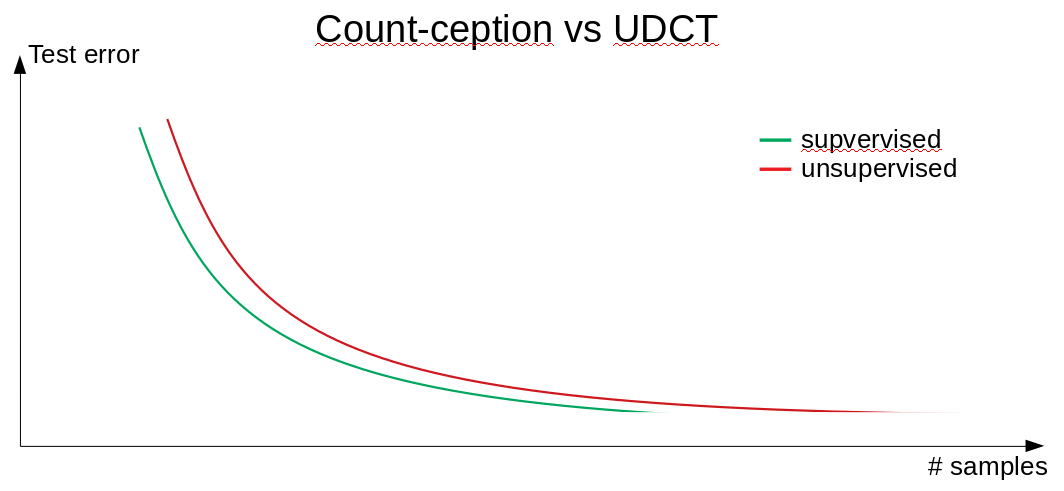
\includegraphics[width=\textwidth]{Figures/sup_vs_unsup.png}
				\captionof{figure}{Expected performance of the supervised method (count-ception) and out unsupervised method.}
				\label{fig:s_vs_un}
			\end{Figure}
		
			\begin{Figure}
				\centering
				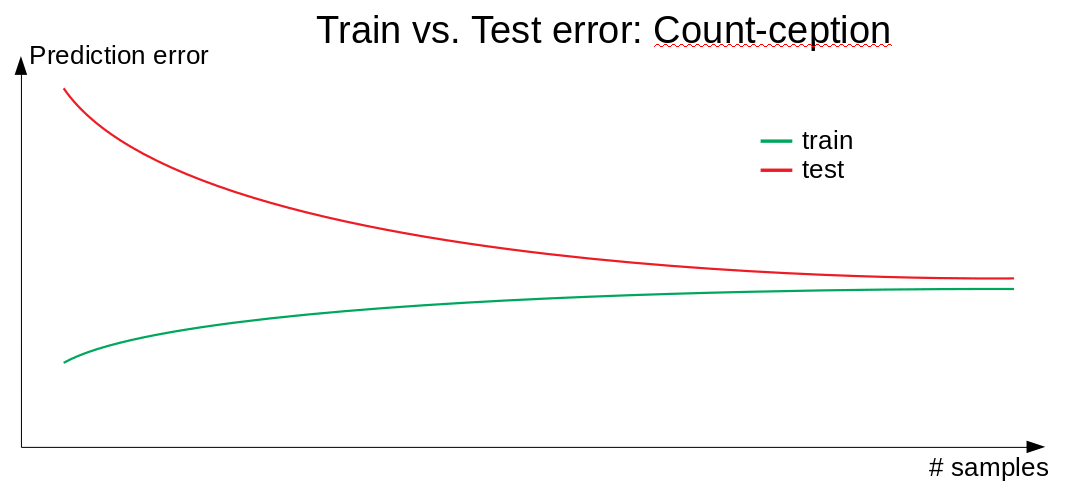
\includegraphics[width=\textwidth]{Figures/train_vs_test_CC.png}
				\captionof{figure}{Qualitative behaviour of the train and test loss for a supervised method.}
				\label{fig:s_vs_un}
			\end{Figure}
			
		\end{multicols}
		
		\begin{multicols}{2}
		
			\begin{Figure}
				\centering
				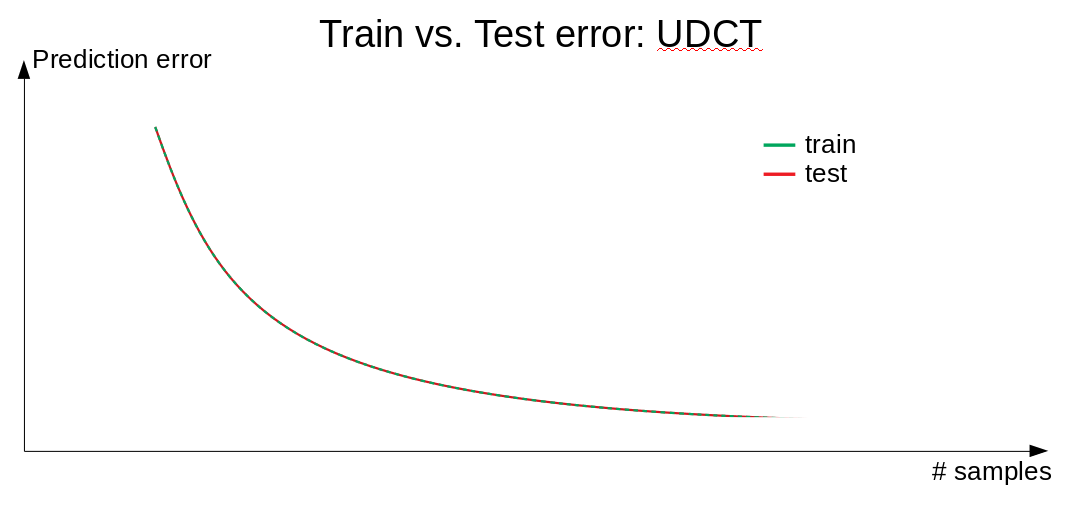
\includegraphics[width=\textwidth]{Figures/train_vs_test_UDCT.png}
				\captionof{figure}{Expected relationship between train and test loss for the UDCT method benchmarked in this thesis.}
				\label{fig:countception}
			\end{Figure}
		
			\begin{Figure}
				\centering
				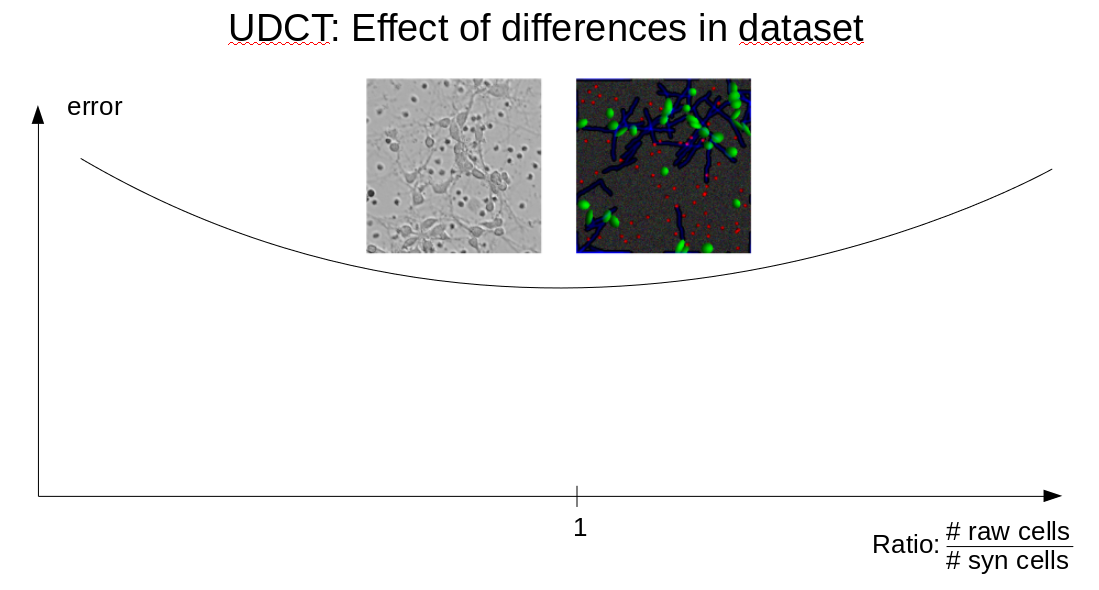
\includegraphics[width=\textwidth]{Figures/ratio.png}
				\captionof{figure}{We suspect that the accuracy of the modified cycleGAN depends on how similar the synthetic data (example image on right side) and the raw data (example image on left side) is. We would like to test this by changing the number of cells in the synthetic dataset. The hypothesized curve is plotted.}
				\label{fig:ratio}
			\end{Figure}
			
		\end{multicols}
		
		Optionally: If there is time left in the project, we would like to investigate how important similar datasets are. We suspect that it is important to have similar datasets. However, this does not need to hold true. To test this, we propose changing the number of neurons in the synthetic dataset and see what effect it has on the prediction error. We suspect that the prediction error behaves as shown in Fig.4.
			
		
	
	\subsection*{Time line}
	
		In total, 280h need to be spend on the project. The third row is a suggestion of how the time could be spend based on requests made by Karthik.
		\begin{figure}[h!]
			\centering
			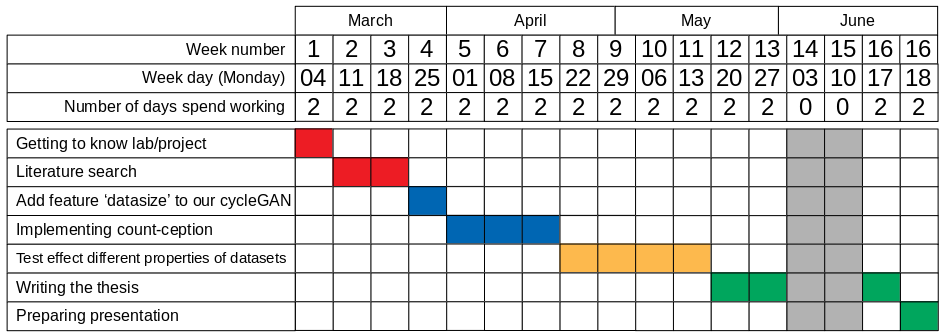
\includegraphics[width=0.9\textwidth]{190303_schedule.png}
		\end{figure}

\end{document}